\documentclass[paper=a4, fontsize=10pt]{scrartcl} % A4 paper and 11pt font size

\usepackage[T1]{fontenc} % Use 8-bit encoding that has 256 glyphs
\usepackage{fourier} % Use the Adobe Utopia font for the document - comment this line to return to the LaTeX default varía la letra de la fuente, poniéndola más gruesa. 
\usepackage{graphicx} % gráficos
\usepackage[spanish]{babel} % English language/hyphenation
\usepackage{amsmath,amsfonts,amsthm} % Math packages
\usepackage[utf8]{inputenc}
\usepackage{lipsum} % Used for inserting dummy 'Lorem ipsum' text into the template
%\usepackage{upgreek} % quitar cursiva a letras griegas
\usepackage{parskip} % suprime sangria 
\usepackage[usenames]{color}
\usepackage[dvipsnames]{xcolor}
\usepackage{siunitx}
\usepackage[colorlinks]{hyperref} % resaltar links


\newcommand{\horrule}[1]{\rule{\linewidth}{#1}} % Create horizontal rule command with 1 argument of height

\title{	
\normalfont \normalsize 
\textsc{Universidad de Los Andes \\
Posgrado en Física Fundalmental \\  Astronomía Extragaláctica y Cosmología} \\ Dra. Fabiola Hernández \\ [25pt] % Your university, school and/or department name(s)
\horrule{0.5pt} \\[0.4cm] % Thin top horizontal rule
\huge Galaxias, relaciones de escalas y distancias extragalácticas \\ % The assignment title
\horrule{2pt} \\[0.5cm] % Thick bottom horizontal rule
}

\author{Margionet Fabiola D\'iaz} % Your name

\date{\normalsize\today} % Today's date or a custom date

\begin{document}

\maketitle % Print the title

%----------------------------------------------------------------------------------------
%	PROBLEM 1
%----------------------------------------------------------------------------------------

\section{Tipos de galaxias y relaciones de escalas}

{\bf{1.1)}} La magnitud absoluta de M101, una galaxia Sc, es $-21.51$ en la banda B. \label{ex:1.1} 

\vspace{0.5cm} 


 
{\bf{[a.]}} Estime el radio para el cual el brillo superficial alcanza el valor $25 \, mag/arcsec^2$ en la banda B.

{\bf{R.}} Para el caso de galaxias espirales, se puede elegir un radio fijo al cual poder estimar la relación masa-luminosidad $M/L$. Esto es debido a que la masa de la galaxia no puede ser conocida con exactitud, pues no conocemos la extensión del halo de materia oscura. De esta manera, para un brillo superficial de $25 \, mag arcsec^{-2}$: 

\begin{equation} \label{eq:1.1}
\log \left(\frac{R_{25}}{kpc} \right) = -0.249 \, M_B - 4.00,
\end{equation}

donde al aplicar la propiedad de los logarítmos: $\log_{10} x = y \Rightarrow x = 10^y$, es posible despejar de \eqref{eq:1.1} $R_{25}$

\begin{equation*}
\left(\frac{R_{25}}{kpc} \right) = 10^{(-0.249 \, M_B - 4.00)},
\end{equation*}

y con una magnitud absoluta de $M_B = -21.51$ para M101 

\begin{equation*}
R_{25} = 10^{[-0.249 \, (-21.51) - 4.00]} kpc,
\end{equation*}

\begin{equation} \label{eq:1.2} 
R_{25} = 22.7 \, kpc.
\end{equation}



\vspace{0.4cm} 


{\bf{[b.]}} Estime la velocidad de rotación de M101.

Para una galaxia espiral $Sc$ la velocidad máxima de rotación viene dada por la siguiente relación: 

\begin{equation} \label{eq:1.3}
M_B = -11.0 \, \log \left(\frac{V_{\text{máx}}}{kms^{-1}} \right) + 3.31,
\end{equation}

y despejando la velocidad máxima de esta última relación 

\begin{align*}
M_B - 3.31 & = -11.0 \, \log \left(\frac{V_{\text{máx}}}{km \,s^{-1}} \right), \\
\\
\log \left(\frac{V_{\text{máx}}}{km \, s^{-1}} \right) & = - \left(\frac{M_B - 3.31}{11.0} \right), \\
\\
V_{\text{máx}} & = \left[ 10^{-(M_B -3.31)/11.0} \right] km \, s^{-1}.
\end{align*}

Finalmente, 

\begin{equation} \label{eq:1.4}
V_{\text{máx}} = 180.4 \, km\, s^{-1}. 
\end{equation}
\vspace{0.3cm} 

{\bf{[c.]}} Calcule la relación $M/L$ para M101 y compare con los valores dados en la literatura.

Para la luminosidad, usando la relación

\begin{equation} \label{eq:1.5}
M_B = M_{Sun} - 2.5 \, \log \left(\frac{L}{L_{\odot}} \right),
\end{equation}

donde $M_{Sun}$ es la magnitud absoluta del Sol, cuyo valor es de $4.74$ se tiene 

\begin{align*}
M_B - M_{Sun} & = -2.5 \, \log \left(\frac{L}{L_{\odot}} \right),\\
\\
\log \left(\frac{L}{L_{\odot}} \right) &= - \left(\frac{M_B - M_{Sun}}{2.5} \right), \\
\\
L & = \left[ 10^{-(-21.51 - 4.74)/2.5} \right] L_{\odot},
\end{align*}

finalmente, 

\begin{equation} \label{eq:1.6}
L = 3.16 \times 10^{10}  L_{\odot}. 
\end{equation}

De la misma manera, hallando la masa encerrada para un radio $R_{25}$, primero es necesario llevar el radio \eqref{eq:1.2} a las unidades correctas. Así, como $1 \, pc= 3.0857 \times 10^{16} m$,

$$ R_{25} = \frac{(22. 7 \times 10^3 \, pc)(3.0857 \times 10^{16} m)}{1 \, pc},$$

\begin{equation} \label{eq:1.7}
R_{25} = 7.00 \times 10^{20} \, m. 
\end{equation}

Transformando también la velocidad máxima \eqref{eq:1.4} a las unidades adecuadas: 

\begin{equation} \label{eq:1.8}
V_{\text{máx}} = 180.4 \times 10^3 m\, s^{-1}.
\end{equation}

Se sigue 

\begin{equation} \label{eq:1.9}
M = \frac{V_{\text{máx}}^2 R_{25}}{G}, 
\end{equation}
 
 con $G$ siendo la constante de gravitación universal $G = 6.67 \times 10^{-11} m^3 s^{-2}$, sustituimos todos lo valores en \eqref{eq:1.9} 
 
\begin{align*}
 M & = \frac{(180.4 \times 10^3 m \, s^{-1})^2 (7.00 \times 10^{20} \, m)}{6.67 \times 10^{-11} m^3 s^{-2} kg^{-1}}, \\
M & = 3.41 \times 10^{41} \,kg,
\end{align*}

que, en unidades solares,

\begin{equation} \label{eq:1.10}
M = 1.65 \times 10^{11} \, M_{\odot}.
\end{equation}
\vspace{0.3cm} 

Finalmente, usando los resultados de la masa y la luminosidad, \eqref{eq:1.6} y \eqref{eq:1.10}, 

\begin{equation*} 
\frac{M}{L} = \frac{1.71\times 10^{11} \, M_{\odot}}{3.16 \times 10^{10}  L_{\odot}},
\end{equation*}

así

\begin{equation} \label{eq:1.11}
\frac{M}{L} = 5.22 \frac{M_{\odot}}{ L_{\odot}}.
\end{equation}

Comparando el resultado \eqref{eq:1.11} con el valor promedio  encontrado en la literatura de la relación masa-luminosidad para una galaxia Sc de $2.6 \, M_{\odot}/L_{\odot}$, se aprecia que el valor obtenido es casi el doble del valor promedio, lo cual se le atribuye a que la galaxia espiral M101 es una galaxia compuesta no solo de materia luminosa sino que también posee un halo de materia oscura, y de aquí que M101 tenga una alta relación $M/L$. 

 
{\bf{{1.2)}}} La galaxia M31 tiene aproximadamente $350$ cúmulos globulares (GC).



{\bf{[a.]}} Si su magnitud visual absoluta es de $-21.7$ calcule la abundancia específica de GC.

{\bf{R.)}}

La abundancia específica de cúmulos globurales viene definida como

\begin{equation} \label{eq:1.12} 
S_N = N_t \frac{L_{15}}{L_V} = N_t 10^{0.4(M_V +15)},
\end{equation}

donde $N_t$ es el número de cúmulos globulares en la galaxia, $L_V$ representa la luminosidad de la galaxia, y $L_{15}$ la luminosidad de referencia correspondiente a una galaxia de magnitud $M_V=-15$. En el caso de la galaxia M31 el número de cúmulos es $~350$. Susitituyendo en \eqref{eq:1.12}

\begin{align*}
S_N = 350 \, 10^{0.4(-21.7+15)},
\end{align*}

\begin{equation} \label{eq:1.13}
S_N = 0.73. 
\end{equation}



 {\bf{[b.]}} NGC 3311 es una galaxia cD con un estimado de $17000$ GC y una magnitud visual absoluta de $-22.4 \,$ mag. Estime la frecuencia específica de GC en esa galaxia.

{\bf{R.)}}  De la misma manera, usando la ec. \eqref{eq:1.12}, para la galaxia cD se tiene 


\begin{align*}
S_N = 17000 \, 10^{0.4(-22.4+15)}, \\
\end{align*}
 así, la frecuencia específica para NGC 3311 es de 
 
\begin{equation} \label{eq:1.14}
S_N = 18,6. 
\end{equation}



{\bf{[c.]}} Discuta el problema de GC desde el punto de vista estadístico tomando en cuenta que las galaxias cD son producto de fusiones de galaxias elípticas ya formadas.

{\bf{R.)}} La cantidad de cúmulos globulares parece ser mayor en galaxias tipo tempranas que en las tipo tardías, y se cree que su número incrementa con la luminosidad total galáctica. Por otro lado, las gigantes cD son galaxias muy brillantes y se encuentran en centros de cúmulos de galaxias. Sobre su formación se dice que son el resultado de la fusión de varias galaxias pequeñas con la galaxia más brillante del cúmulo en el centro. Estas galaxias se caracterizan pues por ser muy luminosas, con un alto brillo superficial en su centro. De esta manera, al ser el número de cúmulos globulares dependiente de la luminosidad, esto sugiere que es lógico pensar que estos cúmulos de estrellas son más probables encontrarlos en galaxias de alta luminosidad como las cD. 

\vspace{0.3cm} 

{\bf{[d.]}} ¿Qué es la abundancia específica de GC? 


{\bf{R.)}} La abundancia específica es una manera de contabilizar la cantidad de cúmulo globulares en una galaxia de luminosidad $L_V$ y magnitud absoluta $M_V$, con respecto a una galaxia estándar, cuya magnitud absoluta en la banda V es de $- 15$ mag. Para galaxias con una alta luminosidad (y aproximadamente masa) la frecuencia específica es más alta. 


 
\vspace{0.5cm}

{\bf{1.3)}} NGC 2639 es una galaxia Sa con una velocidad rotatoria máxima medida de $324 \, Km s^{-1}$
y una magnitud aparente $B = 12.22 \,$  mag (una vez hecha la corrección por extinción),

\vspace{0.3cm} 

{\bf{[a.]}} Estime su magnitud absoluta a partir de la relación Tully-Fisher.

{\bf{R.)}} Para una galaxia $Sa$, la magnitud absoluta de NGC 2639 puede ser determinada por 

\begin{equation} \label{eq:1.15}
M_B = -9.95 \, \log \left(\frac{V_{\text{máx}}}{kms^{-1}} \right) + 3.15.
\end{equation}

Si la velocidad máxima de la galaxia es $V_{\text{máx}} = 324 km\, s^{31}$ se tiene 

$$M_B = -9.95 \, \log \left(\frac{324 km\, s^{-1}}{kms^{-1}} \right) + 3.15,$$ 

\begin{equation} \label{eq:1.16}
M_B = -21.8 \, mag.
\end{equation}

{\bf{[b.]}} ¿Cúal es el radio de la galaxia para un nivel de brillo superfcial de $25 \, B-mag -arcsec^2$?

Conocida la magnitud absoluta  $M_B$, el radio correspondiente a un brillo superficial de $25 \, mag \, arcsec^{-2}$ puede ser determinado de la misma manera que en el ejercicio (\ref{ex:1.1}) 

\begin{align*} 
log \left(\frac{R_{25}}{kpc} \right) = -0.249 \, M_B - 4.00, \\
R_{25} = 10^{[-0.249 \, (-21.8) - 4.00]},
\end{align*} 

obteniéndose 

\begin{equation} \label{eq:1.17}
R_{25} = 26.8 \, kpc.
\end{equation}

 

{\bf{[c.]}}  Encuentre la masa de NGC 2639 encerrada en el interior de ese radio. Expréselo en masas solares.

Calculado el radio, vamos a determinar la masa encerrada de la ec. \eqref{eq:1.9}, donde primero es necesaria las adecuadas unidades para $R_{25}$, 

$$ R_{25} = \frac{(26.8 \times 10^3 \, pc)(3.0857 \times 10^{16} \, m)}{1 \, pc},$$

\begin{equation} \label{eq:1.18}
R_{25} = 8.27 \times 10^{20} \, m.
\end{equation}

Con $V_{\text{máx}} = 324 \times 10^3 \,m$

\begin{align*}
 M & = \frac{(324 \times 10^3 m\, s^{-1})^2 (8.27 \times 10^{20} \, m)}{6.67 \times 10^{-11} m^3 s^{-2} kg^{-1}}, \\
 M_{enc} & = 1.30 \times 10^{42} \, kg, 
 \end{align*}
 que, en masas solares 

 \begin{equation} \label{eq:1.19}
R_{25} = 6.50 \times 10^{11} \, M_{\odot}.
\end{equation}
 
{\bf{[d.]}} ¿Cúal  es la luminosidad de la galaxia en la banda B? Expréselo en luminosidades solares.

\vspace{0.4cm}

De ec. \eqref{eq:1.5}, la luminosidad para la galaxia espiral NGC 2639 

$$ L = 10^{[- (-21.8 -4.74)/2.5]} \, L_{\odot},$$

$$L = 4.13 \times 10^{10} \,  L_{\odot}.$$

{\bf{[e.]}} Calcule la relación masa-luminosidad para NGC 2639 en la banda B dentro del radio $R_{25}$ ¿Cómo es ese valor en comparación con la literatura?

\vspace{0.3cm}

Una vez determinada tanto la masa como la luminosidad, podemos calcular la relación $M/L$

\begin{equation*} 
\frac{M}{L} = \frac{6.50 \times 10^{11} \, M_{\odot}}{4.13 \times 10^{10} \, L_{\odot}},
\end{equation*}

\begin{equation} \label{eq:1.20}
\frac{M}{L} = 15.7 \frac{M_{\odot}}{ L_{\odot}}.
\end{equation}

El valor promedio encontrado de galaxias espirales tipo Sa para la relación masa-luminosidad es de $~ 6.2 \, M_{\odot}/L_{\odot}$, que al ser comparado con el resultado obtenido en ec. \eqref{eq:1.20}, se observa una alta discrepancia. De nuevo, una alta relación masa-luminosidad indica que la galaxia espiral NGC 2939 está compuesta de materia no luminosa en gran cantidad. Prueba de este gran halo es la velocidad máxima de rotación de la galaxia. 


\vspace{0.5cm}



{\bf{1.4)}} De acuerdo al teorema del virial la dispersión de velocidad radial central está relacionada con la masa y el tamaño de la galaxia por $\sigma^2_r \propto M/R$. Use argumentos similares en la relación Tully-Fisher para mostrar que $L \propto \sigma^4_r$, lo cual es la relación Faber-Jackson.

\vspace{0.3cm}

Del teorema del virial, que básicamente representa la conservación de la energía 

$$E = K + V,$$

donde $K$ es la energía cinética, $K=m v^2$, y $V$ es la energía potencial gravitatoria, $E_V = E_{grav} = - GmM/R^2$, siendo $M$ y $R$ la masa y radio de la galaxia. Por conservación de la energía, y considerando que para galaxias elípticas $\sigma_r >> v_{rot}$, 

\begin{equation} \label{eq:1.21} 
\sigma_r^2 \propto \frac{M}{R},
\end{equation}

se sigue que 


$$ \sigma_r^2 = \frac{GM}{R},$$

\begin{equation} \label{eq:1.22} 
 M = \frac{R \sigma_r^2}{G},
\end{equation}


y utilizando las mismas consideraciones que en la "derivación" de la relación de Tully-Fisher sobre \eqref{eq:1.22}, i.e., multiplicando a ambos lados de la expresión 

\begin{align*}
L M & = \frac{\sigma_r^2 R}{G} L, \\
L & = \frac{1}{M} \frac{\sigma_r^2 R}{G} L,
 \end{align*} 

\begin{equation} \label{eq:1.23} 
L  = \left(\frac{M}{L} \right)^{-1} \frac{\sigma_r^2 R}{G}.
\end{equation}

El brillo superficial promedio se escribe como $\left< I \right> = L/R^2 \Rightarrow R^2 = L/\left< I \right>$ que, sustituido en \eqref{eq:1.23}, se obtiene

\begin{align*}
(L)^2 = \left[\left(\frac{M}{L} \right)^{-1} \frac{\sigma_r^2 R}{G} \right]^2, \\
L^2 = \left(\frac{M}{L} \right)^{-2} \frac{1}{G^2} \frac{L}{\left< I \right>} \sigma_r^4, \\
L = \left(\frac{M}{L} \right)^{-2}  \frac{1}{G^2 \left< I \right>} \sigma_r^4.
\end{align*} 

Finalmente, en el centro de la galaxia, $r=0$, la dispersión de velocidades aumenta con la luminosidad,

\begin{equation} \label{eq:1.24} 
L = \left(\frac{M}{L} \right)^{-2}  \frac{1}{G^2 \left< I \right>} \sigma_0^4,
\end{equation}

donde la relación de masa-luminosidad, $M/L$, y el brillo superficial promedio, $\left< I \right>$, deben ser similares para galaxias elípticas. 

\vspace{0.4cm} 


{\bf{1.5)}} La forma del isocontorno de las galaxias elípticas, representada en coordenadas polares como una serie de Fourier se escribe como:


\begin{equation} \label{eq:1.25} 
a(\theta) = a_0 + a_2cos(2\theta) + a_4cos(4\theta) + ...,
\end{equation}


donde $\theta$ es el ángulo medido en dirección contraria a las agujas del reloj a partir del semieje mayor del elipsoide. 


{\bf{[a.]}} ¿Qué representa cada uno de los tres primeros términos de esta expansión?

\vspace{0.3cm} 

{\bf{R.)}} 

\begin{itemize}
\item $a_0 \rightarrow$ representa la forma de un círculo perfecto, 
\item $a_2 \rightarrow$ asociado a la cantidad de elipticidad $\varepsilon$, 
\item $a_4 \rightarrow$ se asocia con el grado de {\textit{boxiness}}, donde: 
\item[-] Si $a_4 <0$ la superficie {\textit{isophotal}} {\footnote{{\textit{Isophotes}}: contornos en los cuales el brillo superficial de una fuente es constante. Así, e.g., si el perfil de luminosidad de una galaxia es elíptico, sus {\textit{isophotes}} son elipses.}} tiende a ser tipo {\textit{boxy}}. 
\item[-] Si $a_4 >0$ entonces la superficie tiende a ser tipo {\textit{disky}}.

\end{itemize}

\vspace{0.4cm} 

{\bf{[b.]}}   Encuentre una expresión general para $a_2$ escrito en términos de $a_0$ y $\varepsilon$, asumiendo, que todos los términos de orden superior son igual a cero. Definiendo $\epsilon$ como la elipticidad de la galaxia de la siguiente manera: $\varepsilon  = 1 - \beta/\alpha$ , donde $\alpha$ es el semieje mayor y $\beta$ el semieje menor.

\vspace{0.3cm} 

{\bf{R.}} Considerando que órdenes superiores a $a_2$ son iguales a cero, la forma del isocontorno para galaxias elípticas, \eqref{eq:1.25}, resultante es

\begin{equation} \label{eq:1.26} 
a(\theta) = a_0 + a_2cos(2\theta).
\end{equation}

De la relación \eqref{eq:1.26}, dándole valores al ángulo $\theta$ obtenemos 

\begin{table}[htbp]
\begin{center}
\begin{tabular}{|l|l|l|}
\hline
$\theta$ & $cos(2\theta)$ & $a(\theta)$ \\ \hline 
$0$ & $0$ & $a_0 + a_2$ \\ \hline
$\pi/4$ & $0$ & $ a_0$ \\ \hline
$\pi/2$ & $-1$ & $ a_0 - a_2$ \\ \hline
$3\pi/4$ & $0$ & $ a_0$ \\ \hline
$\pi$ & $1$ & $a_0 + a_2$ \\ \hline
$5\pi/4$ & $0$ & $a_0$ \\ \hline
$6\pi/4$ & $-1$ & $ a_0 - a_2$ \\ \hline
\end{tabular}
\caption{\small{Valores del radio de contorno $a$ para diferentes valores de $\theta$.}}
\label{tabla:1}
\end{center}
\end{table}

Del cuadro (\ref{tabla:1}), el valor más grande que se obtiene cuando variamos el ángulo $\theta$ es $a_0 + a_1$ y el menor valor $a_0 - a_2$, valores que corresponden entonces al semieje mayor $\alpha$ y semieje menor $\beta$, respectivamente. Una vez identificados $\alpha = a_0 + a_2$ y $\beta = a_0 - a_2$, de la elipticidad $\epsilon$ se sigue que 

\begin{equation} \label{eq:1.27}
\epsilon = 1 - \frac{\beta}{\alpha}, 
\end{equation}

\begin{align*}
\epsilon & = 1 - \frac{a_0 - a_2}{a_0+a_2}, \\
& = \frac{(a_0+a_2) - (a_0-a_2)}{a_0+a_2}, \\
\epsilon & = \frac{2a_2}{a_0 + a_2},
\end{align*}


y despejando de esta última relación el término relacionado con la elipticidad $a_2$

\begin{align*}
2 a_2 & = \epsilon(a_0 + a_2), \\
& = \epsilon a_0 + \epsilon a_2, \\
2a_2 - \epsilon a_2 & =  \epsilon a_0, \\
a_2 (2 - \epsilon) & = \epsilon a_0, 
\end{align*}

finalmente se encuentra 

\begin{equation} \label{eq:1.28}
a_2 = \frac{\epsilon a_0}{2- \epsilon}.
\end{equation}


{\bf{[c.]}} Realice un gráfico en coordenadas polares de $a$ como función de $\theta$ para una galaxia E4 con $a_0 = 30 \, kpc$ y $a_2$ es el determinado en la parte b. De nuevo asuma que todos los términos de
orden superior son igual a cero. 

\vspace{0.3cm} 

{\bf{R.)}} Para una galaxia E4, la relación entre el semi eje mayor $\alpha$ y el semi eje menor $\beta$ tiene un valor de: 

$$ \frac{\beta}{\alpha} = 0.6, $$

Sabiendo esto y haciendo uso de la relación \eqref{eq:1.27}, para la elipticidad, 

$$ \epsilon = 0.6 - 0.4,$$

\begin{equation} \label{eq:1.29} 
\epsilon = 0.4. 
\end{equation}

Este resultado conduce a poder determinar el valor de $a_2$ de \eqref{eq:1.28}. Se tiene 

\begin{align*}
a_2 & = \frac{\epsilon a_0}{2- \epsilon}, \\
& = \frac{0.4 ( 30 \, kpc)}{2-0.4}, 
\end{align*}

con lo que 

\begin{equation} \label{eq:1.30} 
a_2 = 7.5 \, kpc.
\end{equation}

Regresando al radio de contorno en coordenadas polares, \eqref{eq:1.26}, donde el término $a_4 =0$, lo cual indica que estamos en el caso de una elipse sin desviación. Así, haciendo un gráfico en coordenadas polares de $a(\theta)$  y usando los valores ya determinados arriba de $a_2$ y $a_0$, se obtiene



\begin{figure}[h]
\begin{center}
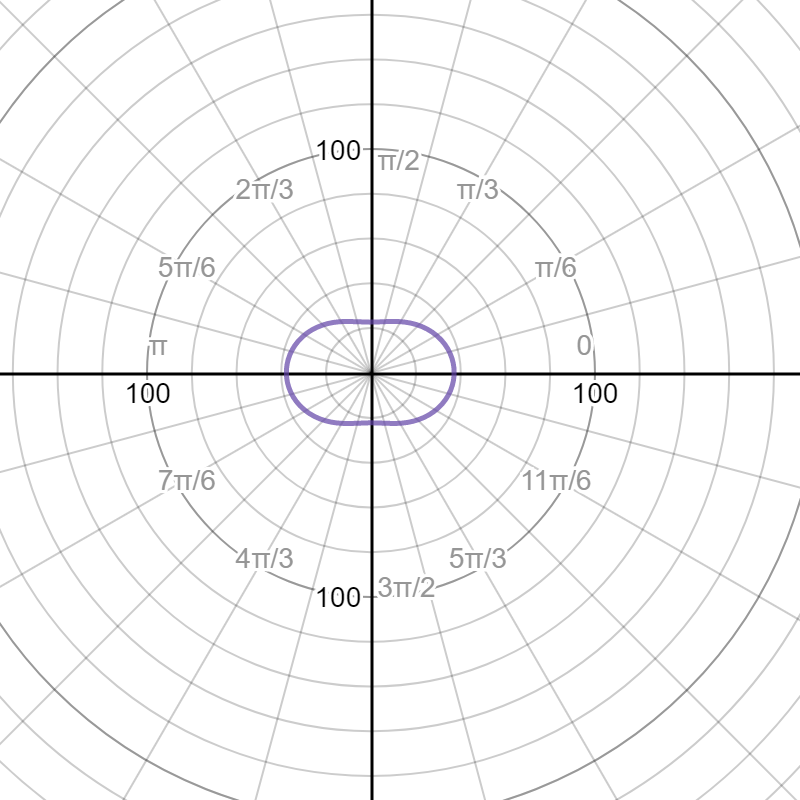
\includegraphics[width=0.6\textwidth]{graf_c_con_lineas}
\caption{\small{Gráfico en coordenadas polares para un $a_0 = 30 kpc$ y un $a_2 = 0.4$. Con $a_4 = 0$, el gráfico muestra una forma elíptica sin desviación.}}
\label{fig:1.1} 
\end{center}
\end{figure}

{\bf{[d.]}} Realice un gráfico en coordenadas polares para la misma galaxia E4 pero con $a_4 = 0.1\,a_0$.


\vspace{0.4cm} 

{\bf{R.)}} Manteniendo invariables los valores de $a_0$ y $a_2$, e incluyendo el término $a_4 = 0.1(a_0) = 3 \,kpc$ en \eqref{eq:1.26}, el cual indica $a_4 > 0$, el caso en donde la tendencia es hacia un {\textit{disky}}, se obtiene 

\begin{figure}[h]
\begin{center}
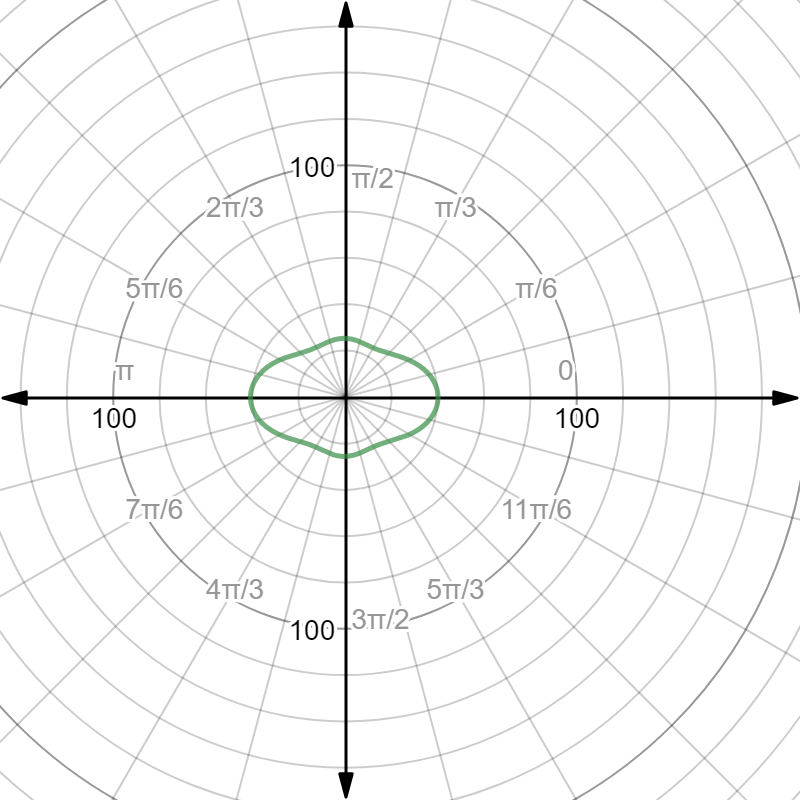
\includegraphics[width=0.6\textwidth]{graf_d_con_lineas}
\caption{\small{Gráfico en coordenadas polares para un $a_0 = 30 \, kpc$, $a_2 = 0.4 \, kpc$ y  $a_4 =3  \, kpc > 0$, caso en el que la deviación con respecto a una elipse tiende a ser tipo {\textit{disky}}.}}
\label{fig:1.2} 
\end{center}
\end{figure}

\newpage 

{\bf{[e.]}} Realice un gráfico en coordenadas polares para la misma galaxia E4 pero con $a_4 = -0.1\,a_0$.


\vspace{0.3cm} 

{\bf{R.)}} Finalmente, manteniendo los valores que en la parte c y d, pero esta vez considerando $a_4 = -0.1a_0 = -3 \, kpc$, i.e., se tiene un $a_4 < 0$.

\begin{figure}[h]
\begin{center}
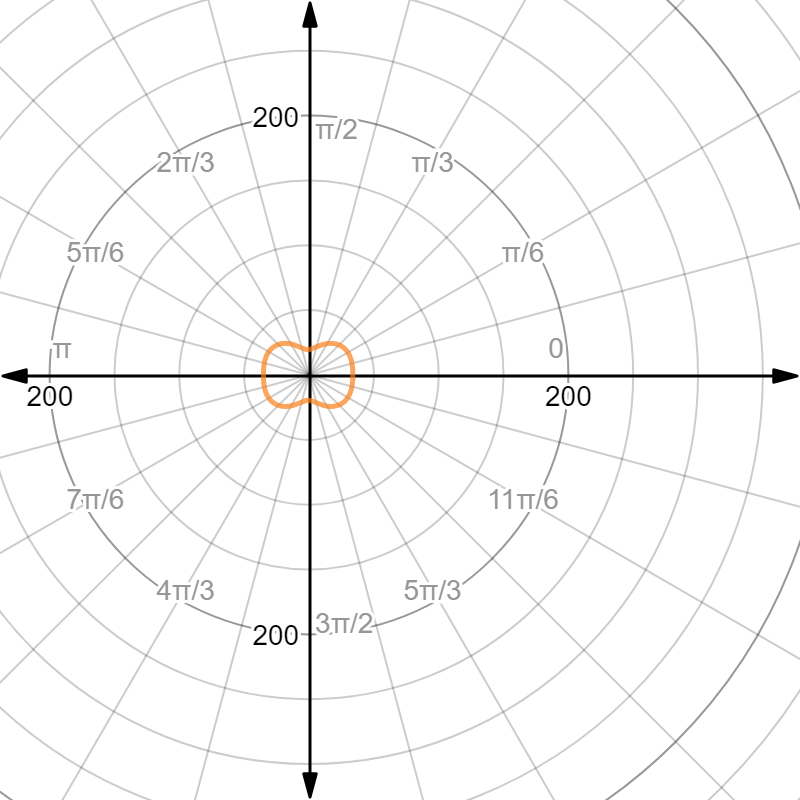
\includegraphics[width=0.6\textwidth]{graf_e_con_lineas}
\caption{\small{Gráfico en coordenadas polares para un $a_0 = 30 kpc$, $a_2 = 0.4$y $a_4 = -3 \, kpc < 0$, donde se observa una tendencia a una forma tipo {\textit{boxy}}. }}
\label{fig:1.3} 
\end{center}
\end{figure}

\newpage 

Superponiendo los tres gráficos se obtiene: 

\begin{figure}[h]
\begin{center}
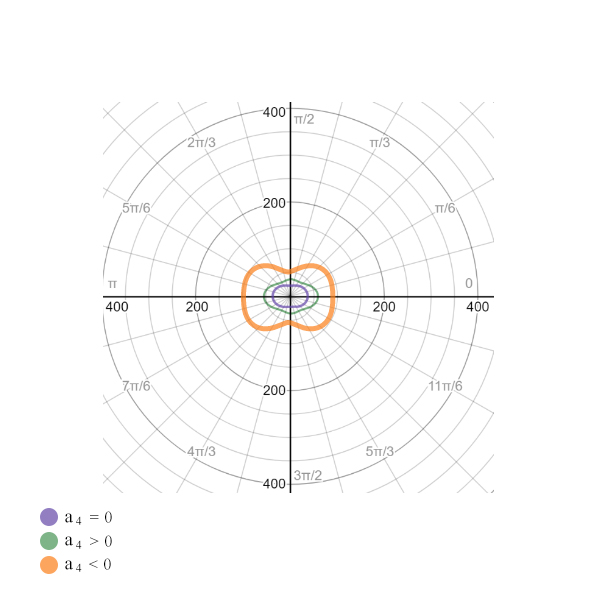
\includegraphics[width=0.8\textwidth]{final_3_}
\caption{Superposición de las figuras (\ref{fig:1.1}), (\ref{fig:1.2}) y (\ref{fig:1.3}), donde se indica de adentro hacia afuera: {\color{Fuchsia}{$a_0=0$}} (elipse sin desviación), {\color{OliveGreen}{$a_4 > 0$}} (desviación tipo {\textit{disky}) y {\color{orange}{$a_4 < 0$}} (tendencia tipo {\textit{boxy}}).}}
\label{fig:1.4} 
\end{center}
\end{figure}



\newpage 

{\bf{[f.]}} Comente sobre los resultados de los últimos dos gráficos ¿Cúal de ellos luce más como una galaxia lenticular? Nota: Todos los gráficos pueden ir en un mismo plot diferenciándolo con colores o estilos de línea. Pueden hacerlos con el graficador que mejor manejen. 

\vspace{0.3cm} 

{\bf{R.)}} Las galaxias lenticulares, $S0$, son una transición entre elípticas y espirales. Esta transición se da en galaxias con tendencias tipo {\textit{disky}}, las cuales representan aproximadamente el $70 \%$ de las galaxias elípticas. Comparando con las últimas gráficas, identificamos a la fig. (\ref{fig:1.2}), con {\color{OliveGreen}{$a_4 > 0$}}, como la galaxia que más se asemeja con una lenticular.
 
\newpage 



\section{Determinación de distancias extragalácticas}

{\bf{2.1)}} Las Cefeidas pueden observarse a una distancia equivalente al Cúumulo de Virgo, y por ser
estándares de luminosidad pueden ser usadas para medir distancias más allá de nuestra Galaxia. En la actualidad los astrónomos usan una muy bien calibrada relación período-luminosidad-color escrita de la siguiente forma:

\begin{equation} \label{eq:2.1} 
M_V = -3.53 \, log_{10}(P_d) - 2.13 + 2.13 (B-V),
\end{equation}

donde $P_d$ es el período de pulsación en unidades de días y $(B-V)$ es el índice de color. Use esta relación en conjunto con la relación período-luminosidad para estimar el rango del índice de color $(B-V)$ para las estrellas variables Cefeidas.

{\bf{R)}} Haciendo uso de la relación Período-Luminosidad calibrada 

\begin{equation} \label{eq:2.2}
M_{\left<V\right>} = -2.18 \log_{10} (P_d) -1.43,
\end{equation}

en conjunto con la relación \eqref{eq:2.1} se va a determinar  el índice de color $(B-V)$ de las Cefeidas Clásicas. Estas estrellas pulsantes tienen períodos de pulsación que van desde $1$ a $50$ días \footnote{Tomado de la tabla 14.1, sec. 14.2, capítulo 14 {\textit{Stellar Pulsation.}}}. Conocido el período de \eqref{eq:2.2} es posible determinar la magnitud absoluta en el visible. 

\vspace{0.2cm} 

\begin{itemize} 

\item Para $P_d = 1$día

\begin{equation*}
M_V = -2.18 \log \, \left(\frac{1 día}{día} \right) -1.43,
\end{equation*}

\begin{equation} \label{eq:2.3} 
M_V =  -1.43 \,mag.
\end{equation}

\item Para $P_d=50$ días:

\begin{equation*}
M_V = -2.18 \log \, \left(\frac{50 día}{día} \right) -1.43,
\end{equation*}

\begin{equation} \label{eq:2.4} 
M_V =  -5.13 \, mag.
\end{equation}

Una vez conocidos los valores de las $M_V$, \eqref{eq:2.3} y \eqref{eq:2.4}, podemos determinar sus respectivos índices de color. Se sigue de \eqref{eq:2.1}

\begin{align*}
M_V + 3.55 \log \, \left(\frac{P_d}{días} \right) + 2.13= 2.13 \, (B-V), \\
(B-V) = \frac{1}{2.13} \left[ M_V +3.55 \log \, \left(\frac{P_d}{días} \right) +2.13 \right].
\end{align*}

\begin{itemize}

\item Para $M_V = -1.43$ y $P_d = 1$ día: 

\begin{equation*}
(B-V) = \frac{1}{2.13} \left[ -1.43 +3.55 \log \, \left(\frac{1 días}{días} \right) +2.13 \right], 
\end{equation*}

\begin{equation} \label{eq:2.5}
(B-V) = 0.33. 
\end{equation}


\item $M_V=-5.13$ y $P_d= 50$ días: 

\begin{equation*}
(B-V) = \frac{1}{2.13} \left[ -5.33 +3.55 \log \, \left(\frac{50 días}{días} \right) +2.13 \right], 
\end{equation*}


\begin{equation} \label{eq:2.6}
(B-V) = 1.33.
\end{equation}

\end{itemize}




\end{itemize}

Finalmente, hemos obtenido que el rango de índice de color $(B-V)$ es:

$$(B-V): 0.33 \hspace{0.3cm} a \hspace{0.3cm} 1.33.$$

\vspace{0.5cm} 

{\bf{2.2)}} La luz producida por la SN 1987A nos da la oportunidad única de medir su distancia (y por lo tanto la distancia a la Gran Nube de Magallanes). La supernova calienta el anillo de gas causando que este brille. El anillo tiene un diámetro angular de $1.66''$ (semieje mayor), se presume que el anillo tiene forma circular pero ladeado con respecto al ángulo de visión. La luz fue recibida con $340$ días de diferencia entre la parte cercana a nosotros del anillo y la lejana.

\vspace{0.3cm}

{\bf{[a.]}} Si en la fotografía $a = 19 \, mm$ y $b = 14 \, mm$, determine el ángulo entre el plano del anillo y el plano del cielo. 

\vspace{0.3cm}

Podemos imaginarnos que si el anillo tuviera un ángulo con respecto a la línea de visión con valores de $0^{\circ}$ o $180^{\circ}$ , lo que veríamos sería un círculo. Del mismo modo, si el ángulo tiene un valor de $90^{\circ}$, veríamos una línea. Para observar una elipse el ángulo tiene que tomar valores $0^{\circ}<\theta < 180^{\circ}$. Asumiendo este último rango, vamos a determinar cuál es el ángulo de inclinación del anillo. De la fig. (\ref{fig:2.1}) imaginemos que estamos mirando al sistema lateral, de forma que hay un ángulo de inclinación entre el anillo y el plano del cielo, el cual es perpendicular a nuestra línea de visión. 

\begin{figure}[h]
\begin{center}
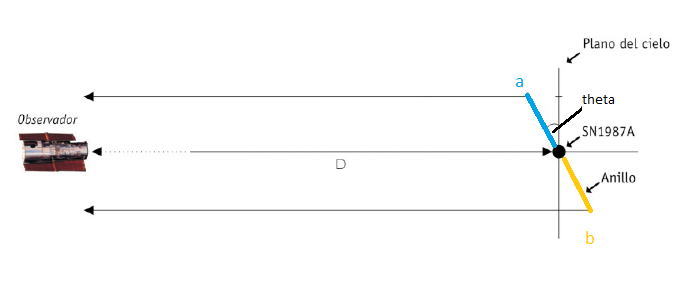
\includegraphics[width=0.8\textwidth]{fig_5_SN}
\caption{\small{Visión lateral al sistema donde se observa que existe un ángulo de inclinación $\theta$ del anillo con respecto al plano del cielo, el cual es perpendicular a la línea de visión del observador.}}
\label{fig:2.1} 
\end{center}
\end{figure}

Teniendo en cuenta esto, podemos determinar el valor del ángulo de inclinación $\theta$ a través de 
$$\cos (\alpha) = \frac{CA}{H},$$

donde $\alpha$ es el ángulo de inclinación $\theta$, el cateto adyacente del triángulo rectángulo que se forma es el semineje menor $b=14\, mm$, y la hipotenusa viene siendo entonces el semieje mayor $a=19 \,mm$. Así, 

\begin{align*}
\cos(\theta) & = \frac{19 \, mm}{14 \, mm}, \\
arccos(\theta) & = \frac{19}{14},
\end{align*} 

finalmente el ángulo de inclinación que se forma entre el anillo y el plano del cielo es de 

\begin{equation} \label{eq:2.7} 
\theta = 47.3^{\circ}. 
\end{equation}

\vspace{0.3cm}

{\bf{[b.]}} Use el retardo temporal para determinar el diámetro del anillo en parsecs. 

\vspace{0.3cm} 

Como ya se mencionó, existe un retardo temporal $t$ entre la parte que, desde la Tierra, vemos que se ilumina primero y el borde más alejado, el cual se ha medido que se ilumina 340 días después. De la fig.  (\ref{fig:2.2}), a esa distancia que hay entre la parte más cerca y la más lejana, la hemos etiquetado como $d_t$. Haciendo uso de $t$, donde sabemos que $1$ día tiene $86400 \,s$ entonces $340$ en segundos es


$$t(s) = \frac{(86400 \,s)(340 \, días)}{1 \, días}, $$

$$ t(s) = 29.4 \times 10^6 \, s.$$ 



Haciedo uso de la velocidad de la luz $c$ se tiene 

\begin{align*}
d_t & = c. t, \\
d_t & = (3 \times 10^8 m\, s^{-1}).(29.4 \times 10^6 \,s),
\end{align*}

escontrándose 

\begin{equation} \label{eq:2.8} 
d_t = 8.82 \times 10^{15} \, m.
\end{equation}

\begin{figure}[h]
\begin{center}
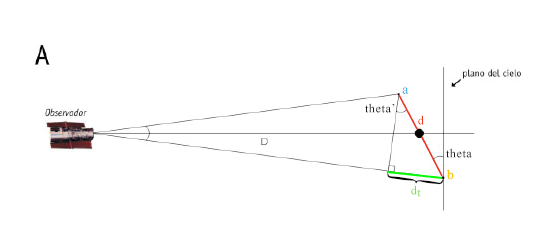
\includegraphics[width=0.8\textwidth]{fig_6_SN}
%\caption{}
\label{fig:2.2} 
\end{center}
\end{figure}

\begin{figure}[h]
\begin{center}
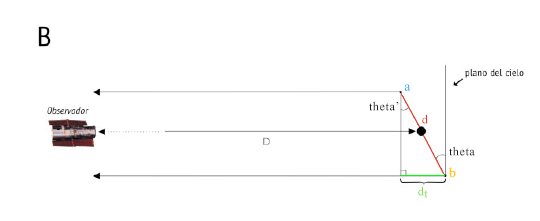
\includegraphics[width=0.8\textwidth]{fig_6b_SN}
\caption{\small{Esquema para la determinación del diámetro real del anillo. En el panel A se muestra la situación real, pero que la distancia a SN1987A sea suficientemente grande, nos pemrite suponer que tanto {\color{ProcessBlue}{a }} como {\color{Goldenrod}{b }} son paralelas, tal como lo muestra el panel B.}}
\label{fig:2.2} 
\end{center}
\end{figure}



Luego de haber determinado la distancia entre la parte más y menos cercana, podemos obtener el diámetro $d$ del anillo. En las figs. (\ref{fig:2.2}) hemos asumido que las líneas que unen a la Tierra con los puntos $a$ y $b$, que son los puntos más y menos cercanos, son paralelas, lo que da pie a considerar que $\theta = \theta'$ ya que el diámetro angular con el que observamos es muy pequeño en comparación con la distancia a la que se encuentra la supernova. De esta manera usando el $\sen(\alpha)$ 

$$\sen(\alpha) = \frac{CO}{H},$$

donde $\alpha = \theta = \theta'$, $CO = d_t$ y la hipotenusa $H = d$. De esta manera 

\begin{align*}
\sen(\theta) & = \frac{d_t}{d}, \\
d & = \frac{d_t}{sen{\theta}}, \\
d & = \frac{8.82 \times 10^{15} \, m}{\sen{47.3^{\circ}}},
\end{align*}

\begin{equation*}
d = 1.20 \times 10^{16} \, m,
\end{equation*}

cuyo valor , en parsecs ($1 \, pc = 3.0857 \times 10^{16} \, m)$ , es de

\begin{equation} \label{eq:2.9}
d = 0.39 \, pc.
\end{equation}

\vspace{0.3cm} 


{\bf{[c.]}} Use trigonometría para encontrar la distancia a SN 1987A.

\vspace{0.3cm} 

Dado el diámetro angular $\delta$, y conocido el cateto opuesto que viene siendo el diámetro del anillo, $d$, podemos, con argumentos trigonométricos estimar  la distancia $D$ a la que se encuentra SN1987A. Transformando el diámetro angular $\delta$ a $\pi $ radianes, 

$$\delta = \frac{(1^{\circ})(1.66'')}{3600''},$$

$$\delta = 0.0005^{\circ}.$$

Y de nuevo, a radianes

$$ \delta = \frac{(0.0005^{\circ})(1 \pi \, rad)}{180^{\circ}},$$

\begin{equation} \label{eq:2.10}
\delta = 8.73 \times 10^{-6} \, rad.
\end{equation}


Como se observa en la fig. (\ref{fig:2.3}) vamos a asumir $d$ como el diámetro de un disco. Es fácil ver de la figura que la distancia $D$ puede escribirse como

$$ \tan(\alpha) = \frac{CO}{CA},$$

donde $\alpha$ no es más que el diámetro angular en radianes, $\delta$, el cateto opuesto  $CO = d$ y nuestra incognita, el cateto adyacente es $CA = D$. Se tiene

\begin{align*}
\tan(\delta/2) & = \frac{d/2}{D}, \\
D & = \frac{d}{2 \tan(\delta/2)}.
\end{align*}

\begin{figure}[h]
\begin{center}
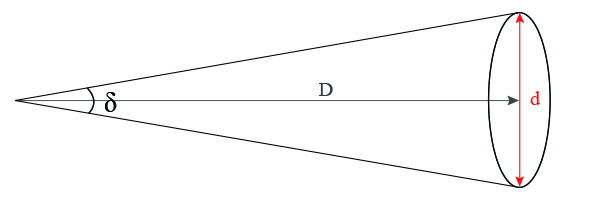
\includegraphics[width=0.7\textwidth]{fig_7_SN}
\caption{\small{Esquema para la determinación de la distancia $D$ a la que se encuentra SN1987A, donde se asume {\color{red}{$d$}} como el diámetro de un disco y donde $\delta$ es el diámetro angular en segundos de arco.}}
\label{fig:2.3} 
\end{center}
\end{figure}


Como $\delta$ es un ángulo muy pequeño, $\tan(\delta/2) \approx \delta/2$. De esta manera 

\begin{align*}
D & = \frac{d}{\delta}, \\
& = \frac{1.20 \times 10^{16} \, m}{8.72 \times 10^{-6} \, rad},
\end{align*}

encontrándose, en metros 

$$ D = 1.38 \times 10^{21} \,m $$ 

y equivalente en kpc, la distancia a SN1987A es

\begin{equation} \label{eq:2.11}
D = 44. 7 \, kpc. 
\end{equation}


\vspace{0.3cm}  

{\bf{2.3)}} Las tres estrellas gigantes rojas más brillantes en la galaxia M101 tienen magnitudes visuales absolutas de $V=20.9 \, mag$. Asumiendo que existe una extinción de $0.3 \, mag$ ¿Cúal es la distancia
a M101? ¿Cómo se compara esto con la distancia de $7.3 \, Mpc$ encontrada usando el método de las Cefeidas? (1 pto).

{\bf{R.}} Siendo la magnitud absoluta de las tres estrellas más brillantes de M101 de $-8$mag, para la longitud de onda en el visible 

\begin{equation}
V = M_V + 5\log \left(\frac{d}{10pc} \right) + A_V,
\end{equation}

donde $V$ es la magnitud aparente visible, $A_V$ la extinción en la misma banda, y $d$ la distancia. Se tiene entonces 

\begin{align*}
5\log \left(\frac{d}{10pc} \right) & = V - M_V - A_V, \\
\log \left(\frac{d}{10pc} \right) & = \frac{V-M_V-A_V}{5}, \\
d & = \left[10^{[20.9-(-8)-0.3]/5}\right]*10,
\end{align*}

finalmente, 

\begin{equation}
d = 5.24 \, Mpc.
\end{equation}

Otro valor encontrado por diferentes métodos arroja una distancia de $6.6 \, Mpc$, lo cual muestra que tanto el método desarrollado en este ejercicio como el métodos de las Cefeidas, diferen por al menos $1 \, Mpc$.
 

\end{document}